% article example for classicthesis.sty
\documentclass[10pt,a4paper]{article} % KOMA-Script article scrartcl
\usepackage{lipsum}
\usepackage[utf8]{inputenc}
\usepackage{amsmath}
\usepackage{url}
\usepackage[nochapters]{classicthesis} % nochapters
\usepackage[pdftex]{graphicx}
\renewcommand{\i}{{\mathrm{i}}}
\renewcommand{\d}{\mathrm{d}}


\begin{document}
    \title{\rmfamily\normalfont\spacedallcaps{Quantum Many-Body Simulations in Haskell}}
    \author{\spacedlowsmallcaps{David Schlegel}}
    \date{01.10.15} % no date
    	
    
    \maketitle
    
    \begin{abstract}
      Applying numerical methods in quantum mechanics has always been necessary in analyzing complex structures of quantum mechanical systems. The technical progress of computer performance has enabled physicists and mathematicians to simulate complex many-body systems. With these methods tangible progress in quantum physics can be made, to analyze quantum phenomena on the level of many-particle interactions. This article focuses on the implementation of numerical methods for many-body simulation in the functional programming language \textbf{Haskell}. Functional programming languages get more and more interesting for physicists through their mathematical way of implementation. In this article simple quantum systems are simulated first and an overview of different numerical methods for solving the Schrödinger equation will be given following an attempt to proceed to many-body systems from simple quantum systems. 
    \end{abstract}
       
    \tableofcontents
    
    \section{Simple Quantum Systems}
   In this chapter simple quantum systems will be studied. Consider a particle in a three-dimensional potential $V(\vec{x})$. The corresponding wave function $\psi(\vec{x}, t)$ is the solution of the Schrödinger equation
   \begin{equation}
  \i \hbar \frac{\partial}{\partial t} \psi(\vec{x}, t) = H \psi(\vec{x}, t) = - \frac{\hbar^2}{2m}	\Delta \psi(\vec{x}, t)+  V(\vec{x}) \psi(\vec{x}, t) \text{,}
   \end{equation}
   where $\Delta$ is the Laplacian differential operator: $\Delta = \frac{\partial^2}{\partial x^2} +\frac{\partial^2}{\partial y^2} + \frac{\partial^2}{\partial z^2} $. For a time-independent potential $V(\vec{x})$ the Schrödinger equation can be formally solved by 
   
   \begin{equation}
     \psi(\vec{x}, t) = \text{U}(t, t_0) \psi(\vec{x}, t_0)   = \exp \left\{ - \frac{\i (t-t_0) }{\hbar} H \right\}  \psi(\vec{x}, t_0) \text{.}
   \end{equation} 
   For a time-dependent potential like an oscillating laserfield, the time evolution of the wave function becomes
   \begin{align}
   \psi(\vec{x}, t) &= \text{U}(t, t_0) \psi(\vec{x}, t_0)  = \hat{\text{T}}_t  \exp \left\{ \frac{\i}{h} \int_{t_0}^t H(\tau) \d \tau \right \}  \psi(\vec{x}, t_0)  \\
   &=  \sum_{n = 0}^\infty \frac{1}{n} {\left( \frac{- \i}{\hbar} \right) }^n \int_{t_0}^t \d t_1\int_{t_0}^t \d t_2 \dots \int_{t_0}^t \d t_n \hat{\text{T}}_t \left\{ H(t_1)H(t_2) \dots H(t_n) \right\} \text{,} \nonumber
   \end{align} 
   where $\hat{\text{T}}_t$ is the time ordering operator. A simple approach is to divide the interval $[0 \dots t]$ into a sequence of $N$ steps so that
   \begin{equation}
   \text{U}(t, t_0) = \text{U}(t, t_{N-1}) \dots \text{U}(t_2, t_1)\text{U}(t_1, t_0)
\end{equation}   and to neglect small deviations of the Hamiltonian in the small interval $\Delta t = t_n - t_{n-1}$.
   
    \subsection{Discretization of the kinetic Energy}
    Dividing the Hamiltonian $H$ into $H = T + V$, the nonlocal kinetic energy operator can be written as
    \begin{equation}
    T \psi(\vec{x}, t) = - \frac{\hbar^2}{2m} \Delta \psi(\vec{x}, t) \text{.}
    \end{equation}
    
    \subsubsection{Method of Finite Differences}
    Taking a grid $(k,l,m)$ in three dimensions, the kinetic energy operator can be approximated by finite differences
    \begin{flalign}
   &  T \psi(\vec{x}, t) =  - \frac{\hbar^2}{2m}  \left(  
     \frac{\psi_{(k+1,l,m)}^n -2 \psi_{(k,l,m)}^n + \psi_{(k-1,l,m)}^n}{\Delta x^2} +\right. \nonumber \\
     & \left . \frac{\psi_{(k,l+1,m)}^n -2 \psi_{(k,l,m)}^n + \psi_{(k,l-1,m)}^n}{\Delta y^2} +
       \frac{\psi_{(k,l,m+1)}^n -2 \psi_{(k,l,m)}^n + \psi_{(k,l,m-1)}^n}{\Delta z^2} \right)
    \end{flalign} with higher order terms $\mathcal{O}(\Delta x^2, \Delta y^2, \Delta z^2 )$ where $n$ represents the discrete time index of the wave function. Considering the time independent Schrödinger equation we can write the operator in one dimension as a matrix satisfying the eigenvalue equation
 \begin{align}
\left[ \begin{pmatrix}
2	& -1	& &  \dots	 & 0      \\
-1	& 2 	&  -1&  & \vdots	  \\
\vdots	& \ddots 	& \ddots &  \ddots & \\
&  &-1 & 2 & -1\\
0 	&   \dots & & -1	 & 2
\end{pmatrix} + V_{kk} \right ]
\begin{pmatrix}\psi_1 \\ \vdots \\ \psi_k \\ \vdots \\ \psi_N \end{pmatrix}
 = E \begin{pmatrix}\psi_1 \\ \vdots \\ \psi_k \\ \vdots \\ \psi_N \end{pmatrix}
\end{align} where $\vec{\psi}$ are the values of the wave function on the evaluation points $x_k$. $V_{kk}$  represents the potential for each $x_k$, thus it is a diagonal matrix.
\par For the example of a particle in a box the potential is
\begin{align} 
V_{kk} = \left\{ \begin{array}{ll}  \infty  \quad \text{for} \quad  k = 0, \; k= N \\  0 \quad \text{else} \end{array} \right. \text.
\end{align}
Solving the above eigenvalue equation yields the eigenfunctions $\psi_n$ with eigenenergies $E_n$. The boundary conditions $V = \infty$ at $k=0$ and $k=N$ are satisfied even when the boundary conditions are left out. An example of the first four eigenstates is shown in \mbox{ figure \ref{fig:eigenfunctions}.}
\begin{figure}[!htb]
	\Huge
	\centering
	\resizebox{!}{0.6\textwidth}{%% Creator: Inkscape inkscape 0.91, www.inkscape.org
%% PDF/EPS/PS + LaTeX output extension by Johan Engelen, 2010
%% Accompanies image file 'eigenfunctions.pdf' (pdf, eps, ps)
%%
%% To include the image in your LaTeX document, write
%%   \input{<filename>.pdf_tex}
%%  instead of
%%   \includegraphics{<filename>.pdf}
%% To scale the image, write
%%   \def\svgwidth{<desired width>}
%%   \input{<filename>.pdf_tex}
%%  instead of
%%   \includegraphics[width=<desired width>]{<filename>.pdf}
%%
%% Images with a different path to the parent latex file can
%% be accessed with the `import' package (which may need to be
%% installed) using
%%   \usepackage{import}
%% in the preamble, and then including the image with
%%   \import{<path to file>}{<filename>.pdf_tex}
%% Alternatively, one can specify
%%   \graphicspath{{<path to file>/}}
%% 
%% For more information, please see info/svg-inkscape on CTAN:
%%   http://tug.ctan.org/tex-archive/info/svg-inkscape
%%
\begingroup%
  \makeatletter%
  \providecommand\color[2][]{%
    \errmessage{(Inkscape) Color is used for the text in Inkscape, but the package 'color.sty' is not loaded}%
    \renewcommand\color[2][]{}%
  }%
  \providecommand\transparent[1]{%
    \errmessage{(Inkscape) Transparency is used (non-zero) for the text in Inkscape, but the package 'transparent.sty' is not loaded}%
    \renewcommand\transparent[1]{}%
  }%
  \providecommand\rotatebox[2]{#2}%
  \ifx\svgwidth\undefined%
    \setlength{\unitlength}{800bp}%
    \ifx\svgscale\undefined%
      \relax%
    \else%
      \setlength{\unitlength}{\unitlength * \real{\svgscale}}%
    \fi%
  \else%
    \setlength{\unitlength}{\svgwidth}%
  \fi%
  \global\let\svgwidth\undefined%
  \global\let\svgscale\undefined%
  \makeatother%
  \begin{picture}(1,0.75)%
    \put(0,0){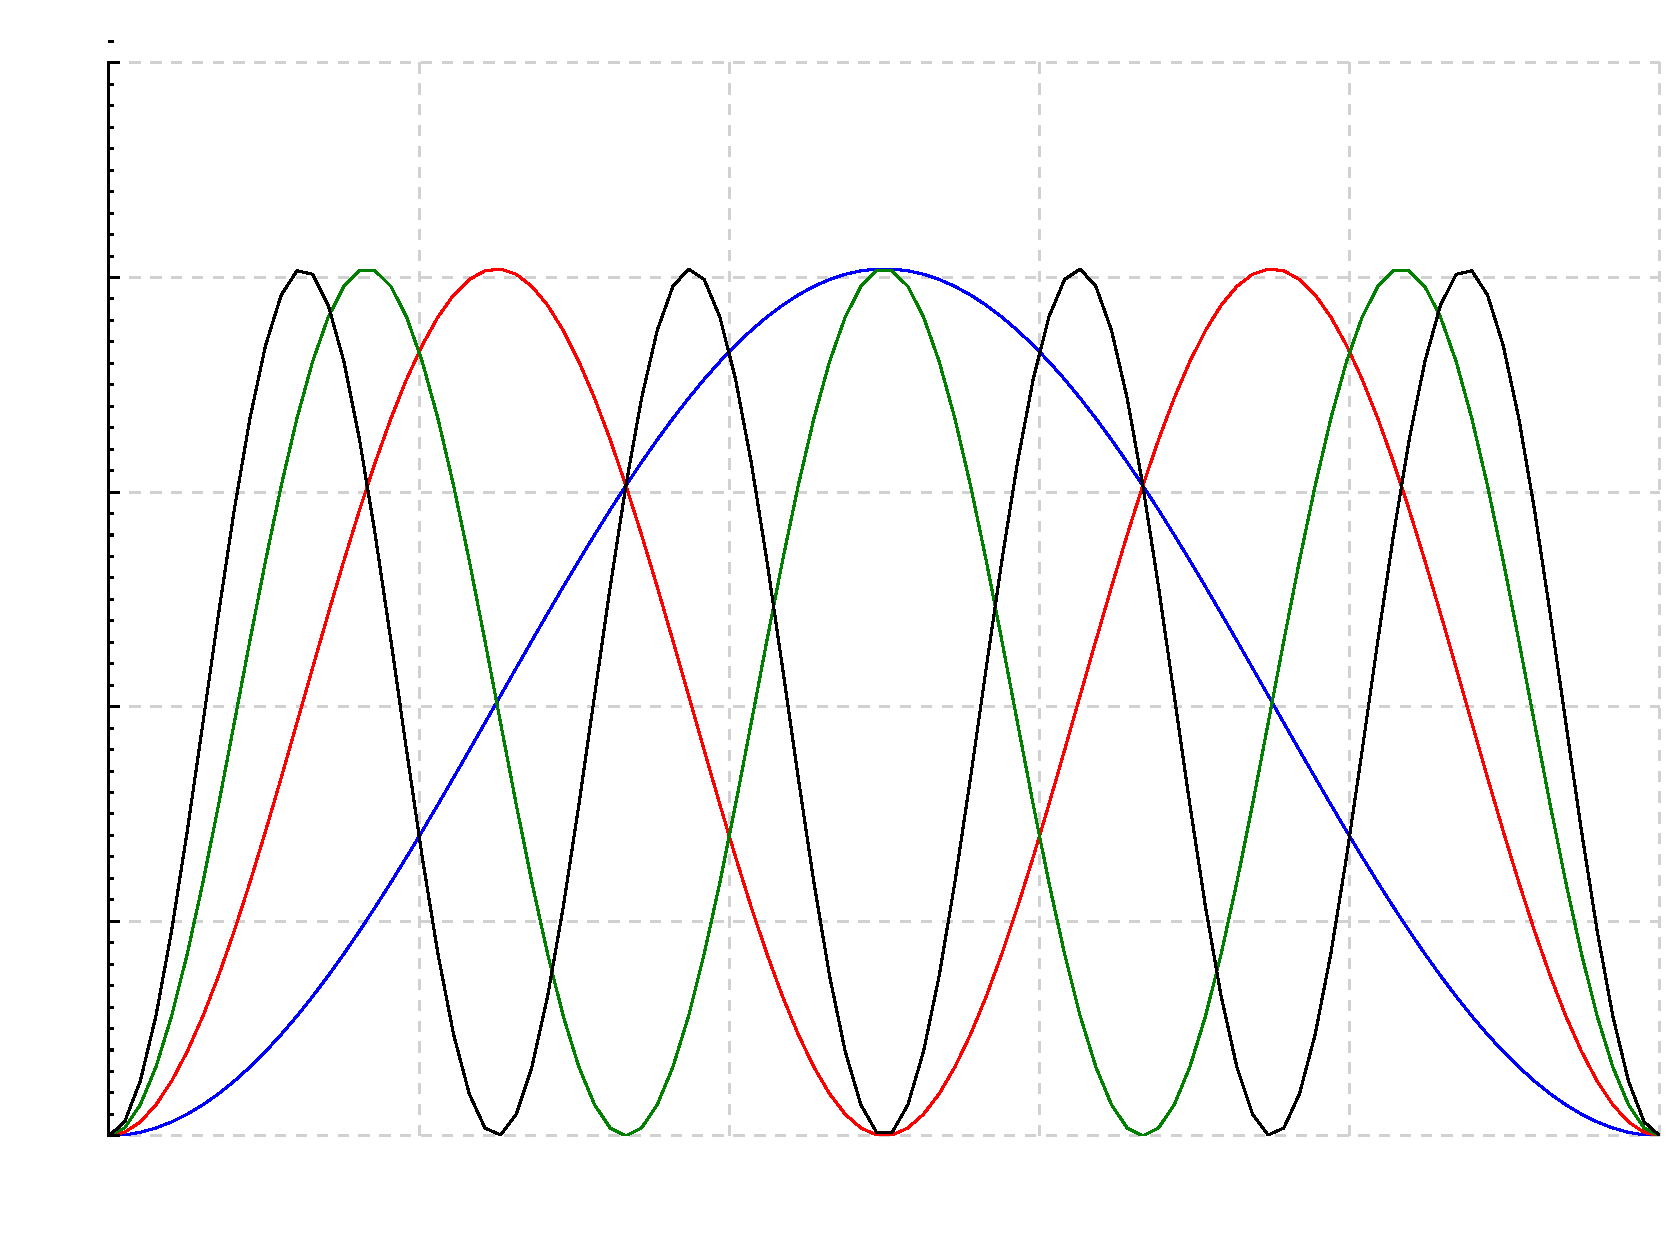
\includegraphics[width=\unitlength,page=1]{figures/eigenfunctions.pdf}}%
    \put(0.004,0.57681454){\color[rgb]{0,0,0}\makebox(0,0)[lb]{\smash{$0.02$}}}%
    \put(0,0){\includegraphics[width=\unitlength,page=2]{figures/eigenfunctions.pdf}}%
    \put(0.0,0.44990405){\color[rgb]{0,0,0}\makebox(0,0)[lb]{\smash{$0.015$}}}%
    \put(0.004,0.32290405){\color[rgb]{0,0,0}\makebox(0,0)[lb]{\smash{$0.01$}}}%
    \put(0.0,0.70690405){\color[rgb]{0,0,0}\makebox(0,0)[lb]{\smash{$0.025$}}}%
    \put(0.004,0.06340405){\color[rgb]{0,0,0}\makebox(0,0)[lb]{\smash{$0$}}}%
    \put(0.004,0.19197949){\color[rgb]{0,0,0}\makebox(0,0)[lb]{\smash{$0.05$}}}%
    \put(0.03773901,0.04840405){\color[rgb]{0,0,0}\makebox(0,0)[lb]{\smash{$0$}}}%
    \put(0.23223901,0.04){\color[rgb]{0,0,0}\makebox(0,0)[lb]{\smash{$0.2$}}}%
    \put(0.41073901,0.03){\color[rgb]{0,0,0}\makebox(0,0)[lb]{\smash{$0.4$}}}%
    \put(0.59823901,0.03){\color[rgb]{0,0,0}\makebox(0,0)[lb]{\smash{$0.6$}}}%
    \put(0.783239,0.03){\color[rgb]{0,0,0}\makebox(0,0)[lb]{\smash{$0.8$}}}%
    \put(0.970739,0.03){\color[rgb]{0,0,0}\makebox(0,0)[lb]{\smash{$1$}}}%
    \put(0.04823902,0.02040406){\color[rgb]{0,0,0}\makebox(0,0)[lb]{\smash{$\psi_1$}}}%
    \put(0.13614134,0.0200705){\color[rgb]{0,0,0}\makebox(0,0)[lb]{\smash{$\psi_2$}}}%
    \put(0.21064144,0.02057045){\color[rgb]{0,0,0}\makebox(0,0)[lb]{\smash{$\psi_3$}}}%
    \put(0.29614145,0.01957047){\color[rgb]{0,0,0}\makebox(0,0)[lb]{\smash{$\psi_4$}}}%
    \put(0.4752763,0.73714841){\color[rgb]{0,0,0}\makebox(0,0)[lb]{\smash{Eigenfunctions}}}%
  \end{picture}%
\endgroup%
}
	\caption{Propability densities for the calculated eigenfunctions $\psi_n$, with the method of finite differences and a grid of $N=100$ for $n = 1,2,3$ and $4$ in one dimension. For simplicity the prefactor $\dfrac{\hbar^2}{2m}$ was set to zero, obtaining non-normalized eigenfunctions.}
	\label{fig:eigenfunctions}
\end{figure} 
To reduce the problem of a particle in three dimensions to a simple matrix equation, the spatial wave function $\vec{\psi}$ can be stacked, to obtain an $N^3$ dimensional vector
\begin{align}
\vec{\psi}_{k,l,m} = \begin{pmatrix}\vec{\psi}_{1,1,m} \\ \vdots \\ \vec{\psi}_{1,N,m} \\ \vdots \\ \vec{\psi}_{N,1,m} \\ \vdots \\ \vec{\psi}_{N,N,m} \end{pmatrix} \text{, through nested vectors.}
\end{align}

    \subsection{A Subsection}
    
    \section{A Section}
    
    % bib stuff
    \nocite{*}
    \addtocontents{toc}{\protect\vspace{\beforebibskip}}
    \addcontentsline{toc}{section}{\refname}    
    \bibliographystyle{plain}
    \bibliography{../Bibliography}
\end{document}
